\documentclass[runningheads]{llncs}
\usepackage{graphicx}
\usepackage{multirow}
\usepackage{verbatim}
\usepackage[toc,page]{appendix}
\usepackage{pdfpages}

\begin{document}


\includepdf[pages=1-]{cover.pdf}

\title{Reasoning with Multi-modal Sensor Data Streams for m-Health Applications}
\author{Anjana Wijekoon\\
Principle Supervisor: Prof. Nirmalie Wiratunga\\
Secondary Supervisors: Prof. Kay Cooper, Dr. Sadiq Sani}
\institute{School of Computing Science and Digital Media, Robert Gordon University, Aberdeen AB10 7GJ, Scotland, UK \\}
\authorrunning{A. Wijekoon}
\maketitle

\section*{Abstract}
Musculoskeletal Disorders (MSD) are chronic conditions with long term impact on individuals and on the society.
Maintaining an active life-style with regular prescribed exercises is crucial for preventing and self-managing MSD. 
Current fitness applications are well versed in recognising limited number of physical activities. 
But, a digital intervention for self-management of MSD require recognition and qualitative assessment of exercises as well as general Human Activity Recognition (HAR).
Drawing on research into HAR; we can see several challenges that must be addressed when developing an end-to-end digital intervention for qualitative exercise recognition: multi-modal sensor fusion; non-invasive HAR; open-ended HAR; and qualitative HAR.
All of which form the basis for research questions that are formulated in this research project.
This research will contribute to the state of the art in machine learning for reasoning with multi-modal sensor streams for human activity recognition.
The overall goal of this research is to build robust qualitative recognition algorithms for exercises that will contribute towards prevention and self-management of MSD. 

\clearpage

\section{Introduction}
\label{sec:intro}
Musculoskeletal Disorders (MSD) are recognised as a primary contributor to disease burden in developed countries~\cite{abajobir2017global}. 
Maintaining a regular self-managed exercise routine while adhering to correct execution is an essential component when living with MSD.
Finding technological solutions for either the prevention or self-management of MSD have been a research area which has emerged over the last few years.
Digital interventions in the form of activity monitoring applications have proven to encourage active lifestyle with the rise of smart devices \cite{fanning2012increasing}. Smart devices collect data that help to keep track of user activities based on sensors that can be worn as well as those that are in the environment. For instance user activities such as walking or jogging are captured with high precision, through automated step counting with accelerometer sensors commonly found in mobile phones or watches. In contrast, keeping track of exercises is completely relied on user input, resulting in poor accuracy and reliability. 

An effective digital intervention for self managing MSD should be capable of interception, recognition and quality assessment of exercises in real-time. 
%Simple sensors on a smart phone are able to identify simple ambulatory activities. 
Exercises can be viewed as a sub category of human activities that comprises of complex sequences of human movements. They require capturing multiple limb movements and need to be captured with strategically placed multiple sensors. Recent literature has looked at activity recognition with multiple homogeneous sensors~\cite{yao2017deepsense,radu2016towards,ordonez2016deep}, but not in a qualitative manner. Evidently there are challenges that arise when reasoning with multi-modal sensors of heterogeneous data types. Specifically we recognise four challenges from our work in the domain of Human Activity Recognition (HAR) that need addressed in order to accomplish end-to-end qualitative recognition (recognition with quality assessment) with multi-modal sensor streams; sensor fusion, non-invasive HAR, open-ended HAR and qualitative HAR. 
While sensor fusion is focused on exploiting multiple sensors for improved recognition performance, non-invasive HAR and open-ended HAR are focusing on improving deployability of HAR algorithms in real-world; the goal of qualitative HAR is to go beyond recognition and assist consumer with correct execution of activities.  

This research will perform a comprehensive literature review on each challenge we plan to explore and introduce new state of the art algorithms for reasoning with multi-modal sensor streams. We affirm that our contributions are not restricted to the domain of exercises but applicable in a wide range of human activity recognition tasks. 
Importantly this work also involves collaboration with the health sciences researchers to collect multiple sensor data for exercises to curate a multi-modal dataset which will be made public for comparative studies in human activity and exercise recognition research. 

\subsection{Challenges in HAR}
Recent literature has recognised a number of challenges that are emerging in the research domain of HAR~\cite{nweke2018deep,baltruvsaitis2018multimodal,wang2018deep}. Here we detail a list of challenges that are specifically applicable for when developing robust qualitative HAR algorithms to use in real-world applications with heterogeneous sensor data types. 

\begin{description}
\item[Sensor fusion:] Sensors are improving everyday providing more accurate and complex data streams. The range of sensors available today for human activity monitoring is not restricted to inertial sensors, Therefore it is significantly important to explore the possibility of combining data streams from diverse group of sensor to improve HAR~\cite{wang2018deep,baltruvsaitis2018multimodal}. Although sensor fusion has been explored with multiple inertial sensor streams (time-series data), limited resources are available on fusion of heterogeneous data streams~\cite{ngiam2011multimodal} as it is challenging to develop shared feature extraction techniques and fusion techniques between multiple data types.

\item[Non-invasive HAR:] Multiple sensors are used in HAR algorithms due to their contribution to improved performance~\cite{radu2016towards}. But it is challenging to deploy a HAR algorithm with complex sensory requirements in a real-world application as sensors can be noisy, malfunctioning or intrusive. Accordingly non-invasive HAR is gaining attention in the HAR research community~\cite{wang2018deep}. The challenge is to build HAR algorithms with optimal performance despite previously mentioned challenges encountered in real-world deployment~\cite{wang2018deep}. 

\item[Open-ended HAR:] HAR algorithms are generally restricted to recognising only the activity classes that were introduced at development. In a real-world application it is desirable if the HAR algorithm is able to transfer its learning in to new activities as they are encountered. This is referred to as open-ended HAR. Maintaining recognition performance as new classes are introduced and recognising new classes with minimal expert interference are challenges when achieving open-ended HAR~\cite{wang2018deep,nweke2018deep}. 

\item[Qualitative HAR:] The ultimate goal of building robust HAR algorithms is to use them in applications that assist users in their daily activities. Assessment of observed activities is essential to build such end-to-end solution. The challenges in qualitative HAR are defining the quality assessment metrics and implementing effective quality assessment algorithms that are generalisable across different domains of human activities~\cite{wang2018deep}. 
\end{description}

\subsection{Research Aims and Objectives}
The overall goal is to introduce novel components for a robust digital intervention that assists self-management of exercise routines. Following an initial literature review to identify the challenge, following four research questions were formulated to achieve this goal. In addition we define five objectives that are expected to meet in order to answer each research question.

\paragraph{Research Questions}
\label{sec:rq}
\begin{enumerate}
\item How to combine multi-modal sensor data streams to improve HAR?
\item How to improve HAR in the presence of noisy, missing or intrusive sensor modalities?
\item How to perform open-ended HAR with minimal expert involvement?
\item How to perform qualitative recognition of activities?
\end{enumerate}

\paragraph{Objectives}
\begin{enumerate}
\item Compile a multi-modal sensor dataset in the domain of exercises.
\item Develop machine learning algorithms to reason with multi-modal sensor data of heterogeneous data types. 
\item Develop algorithms to emulate absent modalities in real-time.
\item Develop algorithms that perform open-ended HAR with minimal expert involvement. 
\item Develop similarity based algorithms for comparing sensor data streams to perform qualitative recognition.
\end{enumerate}

\subsection{Contributions}
\begin{description}
\item[ICCBR 2018:]Improving kNN for Human Activity Recognition with Privileged Learning using Translation Models~\footnote{http://iccbr18.com, published at https://www.springer.com/us/book/9783030010805}
\item[RealX Workshop 2018:]Zero-Shot Learning with Matching Networks for Open-Ended Human Activity Recognition~\footnote{http://www.sicsa.ac.uk/events/sicsa-phd-conference-2018/, published at http://ceur-ws.org/Vol-2151/}\\
Latest of this work with more comprehensive evaluation is currently submitted to AAAI-2019, awaiting notification.
\end{description}

\noindent Rest of the document is structured as follows. Section~\ref{sec:lit} is an introduction to the research domain of HAR and a comprehensive review of literature on each research question we recognised in Section~\ref{sec:rq}. Section~\ref{sec:pro} is a detail description of progress we have made on each objective and Section~\ref{sec:fut} details the planned work for future. Section~\ref{sec:time} illustrates the time management plan for this project. Finally there are 3 appendices; firstly the ICCBR 2018 publication, secondly the draft submitted for AAAI 2019 and finally the RDP planner.  

\clearpage

\section{Literature Review} 
\label{sec:lit}
In this section we first detail the research domain of Human Activity Recognition (HAR) by introducing HAR as a machine learning task, sensors involved, data collections available for research and the most recent recognition algorithms available in literature. Later we look at each research question in detail by performing a comprehensive critical evaluation of existing literature. 

\subsection{Human Activity Recognition}
Reasoning with human activities has been researched in many sub domains. Categorisation of these domains are influenced by the organic grouping of activities we observe in nature~\cite{lara2013survey}. Ambulatory and stationary activities are recognised as the basic human activities. For instance, walking, jogging, and running are categorised as ambulatory activities and standing, sitting or lying are considered stationary activities. Gesture or pose is considered another category of human activities where a single pose may only last a very short period of time while involving only a part of the body. Raising arm, bending, folding arm or pointing hand can be considered as gestures. Activities of daily living (ADL) is a complex category of activities where each activity is a sequence of multiple primary activities. Such activity is performed over a longer period of time compared to a basic activity. For instance, brushing teeth can be considered as an ADL where the person is standing with complex hand movement. Exercises is another complex category of human activities with sequences of movements where cardio exercises, flexibility exercises, resistance exercises are sub categories. 

As a machine learning problem there are different approaches to reasoning with human activities. Recognition is the most common approach where human activities are recognised with sensor data streams. Gait analysis is another approach where identity of a person is determined by their gait sensor data. Qualitative recognition is recognition of activities with quality assessment, where quality can be defined as intensity or precision. In addition, there are multiple approaches to reasoning with human activities with specific medical applications such as sleep analysis or fall detection.

\subsubsection{Sensors}
There are sensors that are encountered frequently when monitoring human activities.
\begin{description}
\item[Inertial Measurement Unit:] Most common body-worn sensors are accelerometers that record the acceleration of movement of the subject. Today accelerometers are coupled with multiple other sensors to introduce extra degree of freedom; known as Inertial Measurement Units (IMU). An IMU consists of three sensing components; a tri-axial accelerometer, a tri-axial gyroscope and a tri-axial magnetometer. The sensors records relative change of acceleration, angular velocity and magnetic field respectively at each axis x, y and z. 
\item[Heart-rate Monitor:] is another frequently used body warn sensor that records the rate of heart beat. It generates a time-series data stream at a constant frequency, recording heart rate at each time-stamp. 
\item[Electro Encephalo Graphic Sensor (EEG):] is used for monitoring electrical brain activity in medical condition detection.
\item[Pressure Sensor:] Pressure sensitive fabric can be used as body-worn sensors or ambient sensors where the fabric is designed in to clothing or integrated in to target surfaces respectively. A pressure mat is a common ambient sensing device that consists of multiple pressure sensors typically arranged in a matrix. Over time a pressure mat generates a sequence of heat-maps that closely resembles a video. 
\item[Depth sensor:] Depth camera is one of the most popular activity monitoring tool, mostly in the gaming industry (for instance, Kinect). At each time-stamp depth camera captures a gray-scale image of the view where gray-scale calculated by the distance between the object and the camera. over time it produces a sequence of gray-scale images.
\end{description}

\subsubsection{Data collections}
\label{sec:data}
There are many datasets complied over the years by researchers to address HAR as a machine learning problem. Table~\ref{table:alldata} summarises some of the most popular datasets. 

\begin{table}
\caption{HAR datasets (A=Accelerometer, G=Gyroscope, M=Magnetometer, P=Pressure sensor, H=Heart-rate sensor, *=Dataset not available publicly) }
\label{table:alldata}
\begin{center}
\begin{tabular}{@{\hspace{5pt}}l@{\hspace{15pt}}l@{\hspace{15pt}}l@{\hspace{5pt}}} 
\hline
Activity Type & Dataset & Sensors \\
\hline
\multirow{3}{*}{HAR}&\cite{chen2015deep}&A \\
&\cite{stisen2015smart}&A and G\\
&SelfBACK~\cite{sani2017learning}&A\\
\hline
\multirow{2}{*}{Gesture}&\cite{bulling2014tutorial}&A and G\\
&PDPoseHD~\cite{ohashi2018attributes}&A, G and M\\
\hline
\multirow{3}{*}{ADL}&Opportunity~\cite{roggen2010collecting}&A, G, M, P, Switches, Microphone \\
&&and Localisation system\\
&PAMAP2~\cite{reiss2012introducing}&A, G, M and H\\
\hline
\multirow{2}{*}{Exercises}&\cite{sundholm2014smart}$^*$&P\\
&\cite{velloso2013qualitative}&A, G and M\\
\hline
\end{tabular}
\end{center}
\end{table}

\subsubsection{Recognition Algorithms}
HAR is modelled as a supervised or semi-supervised pattern recognition problem in machine learning research and we look at how HAR research evolved over the years from traditional machine learning techniques to deep learning algorithms.

\paragraph{Traditional Machine Learning techniques}
Earlier research on HAR was based on pattern recognition using inertial sensor data~\cite{lara2013survey}. HAR was modelled as supervised machine learning problem with algorithms such as Decision trees, Support Vector Machine (SVM), k-Nearest Neighbour (kNN), Artificial Neural Networks (ANN), fuzzy logic and regression models~\cite{lara2013survey}. These algorithms were used with shallow feature representations of sensor data produced by manual feature extraction methods (i. e., feature engineering) such as statistical feature extraction, frequency domain transformations or dimensionality reduction algorithms\cite{lara2013survey}.

The main obstacle of using traditional classification algorithms is the need for manual feature engineering. Recognising the most effective feature representation required several iterations of refinement using processes that are often decoupled from the learning process. This often leads to features that remain domain specific and as a result the classification algorithm misses the opportunity to learn hidden generalisable patterns making them less transferable to new domains. 

\paragraph{Deep Learning techniques}
The development of deep learning algorithms with automated feature engineering techniques such as convolutions and recurrence presented an opportunity to overcome the challenge of manual feature extraction. Most importantly these feature extraction techniques can be coupled with traditional classification algorithms such as SVM or ANN to iteratively improve feature representation toward better classification accuracy~\cite{sani2017learning}. Convolution operations that are capable of learning spatial features~\cite{lecun1990handwritten}, are most often coupled with a one hidden layer ANN, and is known as a Convolution Neural Network (CNN). In contrast recurrence operations are specialised in exploiting temporal dependencies and learning temporal feature representations~\cite{elman1990finding}. 

A pyramid like convolutional architecture was proposed by~\cite{sani2017learning} to evaluate the effectiveness of deep feature representation on classification performance against traditional shallow feature representations. No significant classification performance difference was observed between shallow features and deep features from a less-noisy sensor. But the deep feature extraction techniques were most effective with noisy sensors where the model iteratively learnt to discard noise resulting in improved feature representation. 
Another notable research in deep feature extraction for HAR is by~\cite{ronao2016human}. They evaluate their inverted pyramid like convolutional architecture with two inertial sensor data streams for HAR. Their research shows that CNN outperforms traditional classification algorithms with shallow features. In addition they conclude that a hybrid feature engineering approach is favourable where frequency domain transformation is coupled with the deep convolutions. 
An insightful research was done by~\cite{hammerla2016deep} in the domain of HAR where they evaluate recurrence vs. convolutions as deep feature extraction techniques in different domains of HAR. Their results demonstrate the importance of selecting correct feature extraction technique for each domain of activities. For instance, repetitive activities such as walking or running favour convolutions over recurrence; in contrast activities with natural ordering such as activities of daily living favour recurrence over convolutions. 

In summary, it is evident that deep feature extraction techniques improve classification performance compared to hand-crafted features. Further more a hybrid approach to feature engineering is much more effective for when reasoning with time-series data generated by an inertial sensor. A hybrid (shallow+deep) approach utilises both manual feature engineering techniques such as frequency domain transformation and deep feature extraction techniques such as convolutions. We also identify that the architectures we discussed above are restricted to a homogeneous data type (time-series data) and unable to reason with different types of sensor data. We plan to explore hybrid feature extraction techniques that can adapt to any data format, as they enable classification algorithms to exploit many more sensor types.

\subsection{Sensor Fusion}
Sensor fusion is one of the outstanding challenges in the HAR domain~\cite{wang2018deep,baltruvsaitis2018multimodal}. Research in sensor fusion for HAR is driven by the fact that a single sensor is not capable of capturing human body movements with necessary precision compared to multiple sensors. Accordingly the challenge is to expand recognition models to exploit multiple sensors of different and complex data types.

Fusion architectures with deep learning algorithms have been mainly investigated in the area of reasoning with video, where still images from video are treated as multiple inputs. \cite{karpathy2014large} and \cite{pigou2015beyond} use fusion architectures to classify video by experimenting fusion in different levels of abstractions. \cite{ngiam2011multimodal} using a Random Boltzmann Machine (RBM) as a fusion architecture to reason with audio and video data. 

In the HAR domain \cite{radu2016towards} introduce a deep RBM architecture for sensor fusion of two sensors; an accelerometer and gyroscope, which outperformed several traditional methods with shallow feature representations. More recently \cite{yao2017deepsense} integrated convolutional and recurrence architectures to learn spatial and temporal dependencies from multiple sensors. This fusion architecture was evaluated for HAR with accelerometer and gyroscope sensor data streams and was found to outperform results from \cite{radu2016towards}. DeepConvLSTM is another hybrid deep model introduced by~\cite{ordonez2016deep}. They exploit multiple inertial sensors for feature representation and out-performs CNN architecture and traditional classification algorithms. Fusion of sensor data in different levels of abstractions has been developed for HAR by~\cite{munzner2017cnn} which was evaluated with multiple inertial sensors. 

Literature on sensor fusion architectures reveals that the evaluations however fail to present improvements that are statistically significant to support multiple sensors over a single sensor. More importantly all these algorithms were evaluated on datasets with inertial sensors (time-series data); to the best of our knowledge there have been no research that attempted heterogeneous data fusion in the context of HAR. In addition there is opportunity to improve on informed selection of sensors/features and noise reduction.

\subsection{Non-invasive HAR}
Multiple sensor modalities provide more accurate recognition performance compared to using a single modality~\cite{radu2016towards}. But using minimal sensor configuration is preferred by a consumer as it is more convenient and less invasive. A single non-invasive sensor modality is likely to pick up movement that is both relevant as well as extraneous to the human activity being tracked. Accordingly the classification algorithm performs poorly compared to when more accurate sensors are present. 
Importantly there is no restriction to how many sensors we can use during model development (or at training time). Therefore we explore non-invasive HAR as  learning from multiple sensors during training and deploying with minimal sensors necessary.

Classification models struggle to maintain performance when features are missing after deployment which is the main challenge of this approach. Statistical imputation techniques were developed to generate replacements for missing features~\cite{garcia2009k,little2014statistical} and more recently deep sequence generation techniques are used~\cite{shi2017learning}. Privileged Learning~\cite{vapnik2009new} approach adapted by~\cite{shi2017learning} is using a deep recurrence regression model to generate missing skeleton information from depth sequences. Generative techniques are more advantages in our problem as it exploits the available sensors to generate the missing sensor data. 

Image or video captioning~\cite{yu2016video,vinyals2015show}, language translation~\cite{luong2015multi}, time-series forecasting~\cite{ma2015long} and audio and video reconstruction~\cite{ngiam2011multimodal} are several domain where sequence generation has been successfully implemented by exploring temporal dependencies. In contrast image generation with Generative Adversarial Networks (GAN)~\cite{goodfellow2014generative} and dimensionality reduction with Auto-encoders~\cite{vincent2010stacked} are generative techniques that explore spacial dependencies. Learning to reconstruct missing sensor data is similar to sequence generation, but as we focus on a small window of time, where there are less temporal dependencies to be learnt. In addition, we are planning to influence the sensor data generation with input from available sensors, which makes GANs an unsuitable method as it is unable to generate an output influenced by the input sensor data. The mapping between input and output data in an Auto-encoder is more relevant for sensor data generation; unlike the most common use of Auto-encoders we focus on input and output that are not identical - instead they involve different sensor streams aligned in time. 

\subsection{Open-ended HAR}
The ability to incorporate new activities elegantly into pre-trained models after deployment remains an open challenge~\cite{nweke2018deep}. Accordingly, researchers have recognised the need for open-ended HAR~\cite{kawaguchi20164} with a view to creating robust HAR applications that can be personalised to an individual’s preferred set of activities.
Existing methods reported in literature fall under supervised and unsupervised approaches; where the former relies on some user supervision at deployment whilst the latter relies on concept change detection algorithms to recognise new activities.

Unsupervised methods by nature do not rely on labelling and are naturally suited for open-ended HAR. Incremental updates to the clusters allow integration of new classes as instances are folded-in~\cite{gjoreski2017unsupervised} even after model deployment. However the absence of any supervision means that it is harder to recognise both long and short bursts of new activity classes with a single recognition algorithm. Each activity category requires different sensitivity thresholds to be set depending on their expected activity cyclic length or duration of observed activities. Consequently, recognition is focused on one category at the expense of ignoring the other. Such a mixed range of different activity types requires different sensitivity thresholds to be accommodated.

Recognising classes not seen during training as a supervised learning problem is often referred to as Zero-shot Learning (ZSL). Exploiting semantic knowledge of activities to achieve ZSL is the most common approach seen in literature in both HAR~\cite{liu2011recognizing,cheng2013nuactiv,cheng2013towards} and computer vision~\cite{lampert2009learning,lampert2014attribute} domains. 
An activity-attribute matrix is an example of intermediary semantic knowledge-base used in achieving open-ended HAR~\cite{cheng2013nuactiv,cheng2013towards}. The matrix provides domain expert knowledge which defines a sequence of intermediate-level activity attributes (hence intermediary semantic knowledge-base) describing a high-level exercise class. For instance, a chest-press exercise is described as a sequence of Arms side, Arms curl and Arms forward. This approach was later improved to incorporate temporal aspect of attribute sequence~\cite{cheng2013nuactiv}. The semantic knowledge is integrated in to a Support Vector Machine (SVM) classification algorithm with active learning feedback loop to recognise activities. 
Similar approach is followed in one of the latest industrial pose recognition application~\cite{ohashi2018attributes} which introduces a k-Nearest Neighbour (kNN) based Zero-Shot Learning (ZSL) algorithm. Their semantic knowledge-base is similar to~\cite{cheng2013nuactiv} which defines how a set of intermediary human movements would describe an activity. They use deep convolutional models to predict a set of abstract-level semantic features which are intermediary human movement classes. Thereafter pose recognition involves the mapping of aggregated predictions into a single poses using the knowledge base. 

It is evident that reliance on additional domain knowledge(i.e., knowledge-intensive) is the most established approach to Open-ended HAR. Specifically for open-ended HAR, the manual knowledge acquisition burden is less desirable. Therefore it is important to explore methods that are independent of domain expert knowledge (i.e., knowledge-light).  

\subsection{Qualitative HAR}
Quality assessment is recognised as one of the key challenges that need addressed when building an end to end digital intervention~\cite{wang2018deep}. Qualitative HAR has been defined as the comparison between the user execution and the specification of an activity~\cite{velloso2013qualitative}. Research on qualitative HAR also emphasise that an activity should have an appropriate complexity to perform a qualitative assessment~\cite{velloso2013qualitative}; thus we exclude basic activities such as walking or sitting in this context. Exercises is one of the main categories of human activities that would benefits from qualitative assessment in a real-world applications. Accordingly we look two main approaches present in literature, rule-based systems and multi-class classification. 

One of the traditional approaches to quality assessment is exploiting expert knowledge to define rules of correct execution. This approach has been explored with manually crafted shallow features for rehabilitation exercises~\cite{chen2013rehabilitation}. A classifier is followed by a rule based quality assessment component to recognise and assess quality of an exercise. Their quality assessment problem has two possible outcomes which are correct or incorrect. 
Another rule based system found on literature is for weight-lifting exercises~\cite{velloso2013qualitative}. Their approach use predefined specification of weight lifting exercise execution and define angular details of body joints as rules of correct execution. They detect incorrect execution by measuring the deviation of user execution compared to the rules. 

Interpreting qualitative recognition as a multi-class classification problem is another approach for Qualitative HAR.
This method was adapted in the domain of weight-lifting exercises by~\cite{velloso2013qualitative}. Here the classification classes were derived from one correct execution and multiple incorrect executions. \cite{khan2015beyond} implemented a multi-class classification problem to identify skill level of performing surgery, where the classes are comprised of different skill-levels. Another adaptation of this technique is by~\cite{garcia2011statistical} where the activity intensity is modelled as a multi-class classification problem.

A comparison between two approaches demonstrated that rule-based approach out-performs multi-class classification approach~\cite{velloso2013qualitative}. Although, rule-based approach is knowledge-intensive as it requires domain expert to provide execution specifications and rules; resulting in expense of maintenance and less generalisability.
Data-driven approach facilitate more flexible definition for qualitative recognition via multiple classes. But this is infeasible as it requires an intensive data collecting task to include all correct and incorrect executions per each activity class with sufficient labelled data. 
We recognise qualitative recognition as an important yet challenging domain of HAR. Following the definition of qualitative recognition from~\cite{velloso2013qualitative} we realise that measuring the deviation from specification is open to interpretation. In addition above methods use hand crafted features and there is no evidence seen in literature exploring the advantages of deep learning techniques to address this task to the best of our knowledge. Evidently a comprehensive research effort is required to exploit the state of the art machine learning techniques to address this problem. 
0.990
\clearpage

\section{Progress}
In this section we will discuss the progress we have made with each objective. First we will detail the progress we have achieved with the data collection task (Objective 1), followed by the methodology and datasets we will be using to evaluate outcome of each objective. Next we will succinctly discuss the progress and contributions that were made with objectives 3 and 4. 
\label{sec:pro}
\subsection{Objective 1 - Multi-modal Data Collection for Exercises - MEx}

\begin{figure}[ht]
\centering
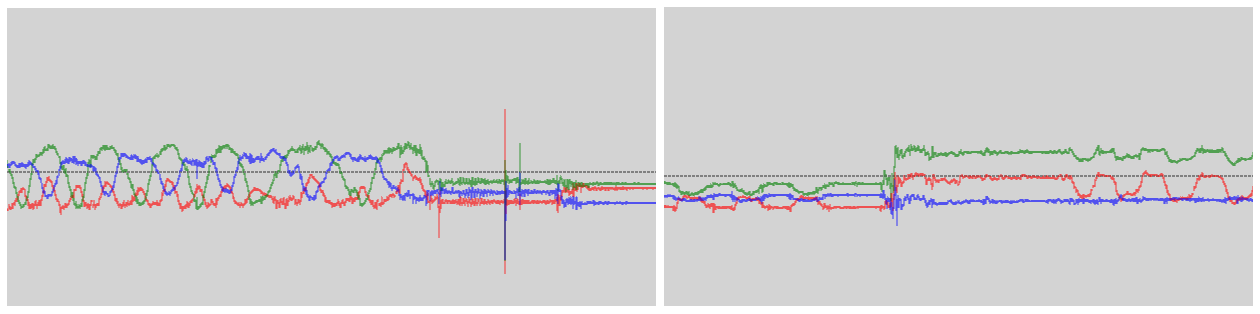
\includegraphics[width=0.8\textwidth]{acc.png}
\caption{3-axial time-series data from accelerometer}
\label {fig:acce}
\end{figure}

\begin{figure}[ht]
\centering
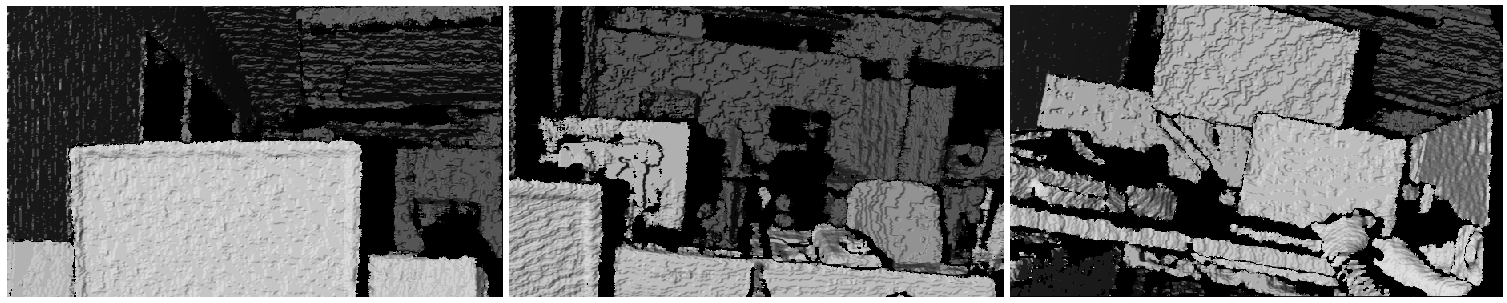
\includegraphics[width=0.8\textwidth]{dpt.png}
\caption{Depth data frames from depth camera}
\label {fig:rgbd}
\end{figure}

\begin{figure}[ht]
\centering
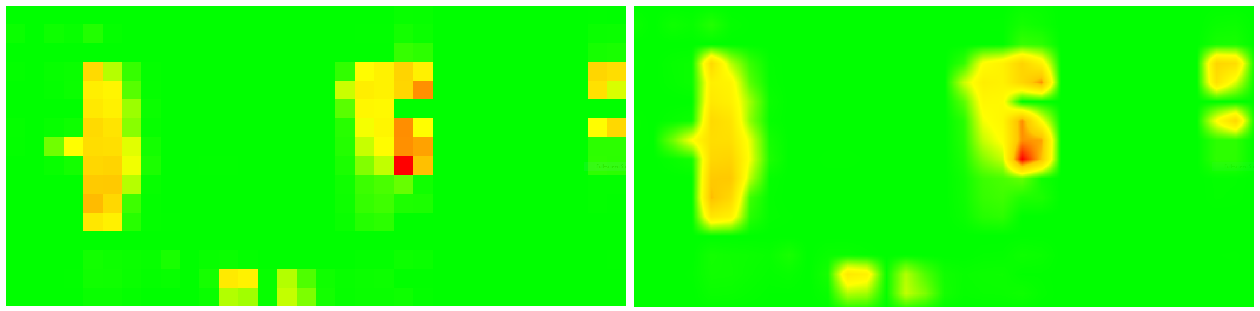
\includegraphics[width=0.8\textwidth]{pm.png}
\caption{Heat-map data frames from pressure map }
\label{fig:pressure}
\end{figure}

Sensor selection for this data collection was influenced by the drawbacks of existing data collections we identified in Section~\ref{sec:data}. Existing datasets in the domain of exercises were either not publicly available, restricted to a single or homogeneous sensor type or restricted to single exercise class. 
Our collection of sensor include 2 accelerometers, depth camera and pressure mat; together they capture different facets of human movements while generating different types of data (time-series, depth sequences and heat-map sequences). We selected seven exercises that are recommended for low-back pain patients; exercises that encourage flexibility and balance. The data collection protocol was approved by the ethics committee from the School of Heath Sciences. 

Data collection is planned for 30 volunteers, each performing 60 seconds of each exercise. A user will contribute roughly seven minutes of sensor data recordings and we will record approximately 3.5 hours of data distributed evenly across seven classes. This is an ongoing task and currently we have collected data with 7 volunteers. After completion, data will be pre-processed to ensure anonymity and disseminated. This \textbf{M}ulti-modal sensor data collection for \textbf{Ex}ercises ``MEx'' will be used to evaluate algorithms we design during the course of this research. 

\subsection{Evaluation Methodology and Datasets}
We evaluate our algorithms with datasets from multiple domains in HAR to verify generalisability. We have selected 4 publicly available datasets and together with MEx there are 5 HAR datasets where classes belong to HAR domains such as ambulatory, stationary, ADL, gesture and exercises. All algorithms will be evaluated with each dataset, where the only exception is objective 5 where qualitative recognition is only applicable for MEx. A detailed description of each dataset can be found in Table~\ref{tbl:data_collections}.

We will perform user hold-out validation, where we will use data from $2/3$ of users as training data and data from $1/3$ of the users as test data. This test strategy emulates a real-world scenario where consumers of the reasoning model is not part of the training dataset. We will repeat each experiment with random user selections and report statistical significance of our results against the most appropriate baselines.

\begin{table}
\caption{Evaluation Datasets}\label{tbl:data_collections}
\centering
\begin{tabular}{@{\hspace{5pt}}l@{\hspace{15pt}}l@{\hspace{15pt}}l@{\hspace{5pt}}}
\hline
Data set&Property&Value\\
\hline
\multirow{7}{*}{$SelfBACK^9$}&Sensors&2 tri-axial accelerometers placed on\\
&&wrist and thigh\\
&Sampling Rate&100Hz\\
&Number of users&49\\
&Activities&9 Activities, Jogging, Sitting, Standing, Lying, \\
&&Walking downstairs, Walking upstairs, Walking\\
&& fast, Walking moderate pace, Walking slow\\
\hline
\multirow{5}{*}{$SelfBACK^6$}&Sensors&A tri-axial accelerometer placed on the wrist\\
&Sampling Rate&100Hz\\
&Number of users&34\\
&Activities&6 Activities, Jogging, Sitting, Standing, Walking, \\
&&Walking downstairs, Walking upstairs\\
\hline
\multirow{9}{*}{PAMAP2}&Sensors&3 Inertial Measurement units (IMU)\\
&Sampling Rate&9Hz\\
&Number of users&10\\
&Activities&18 Activities, Lying, Sitting, Standing, Walking,\\
&&Running, Cycling, Nordic walking, Watching TV,\\
&&Computer work, Car driving, Ascending stairs,\\
&&Descending stairs, Vacuum cleaning, Ironing, \\
&&Folding laundry, House cleaning, Playing soccer, \\
&&Rope jumping, Other (transient activities)\\
\hline
\multirow{10}{*}{HDPoseDS}&Sensors&31 Inertial Measurement units (IMU)\\
&&placed over full body\\
&Sampling Rate&60Hz\\
&Number of users&10\\
&Activities&22 Poses, Standing, Sitting, Squatting,\\
&&Raising arm (L, R), Pointing (L, R), Folding\\
&&arm, Deep breathing, Stretching up, Stretching\\
&&forward, Waist bending,Waist twisting (L, R), \\
&&Heel to back (L, R), Stretching calf (L, R),\\
&&Boxing, Baseball hitting, Skiing, Thinking\\
\hline
\multirow{10}{*}{MEx}&Sensors&2 tri-axial accelerometers placed on the wrist and\\
&&thigh, A pressure mat with 16*32 resolution,\\
&&A depth camera\\
&Sampling Rate&Accelerometer - 100Hz\\
&& Pressure mat - 10Hz\\
&& Depth Camera - 10Hz\\
&Number of users&30 (expected)\\
&Activities&7 Low-back pain exercises, Knee rolling, Bridging\\
&&Pelvic tilt, The clam, Repeated Extension\\ 
&&in lying, Prone punches, Superman\\
\hline
\end{tabular}
\end{table}

\subsection{Objective 3 - Improving feature representations with Translators for Non-invasive HAR}
\begin{figure}[ht]
\centering
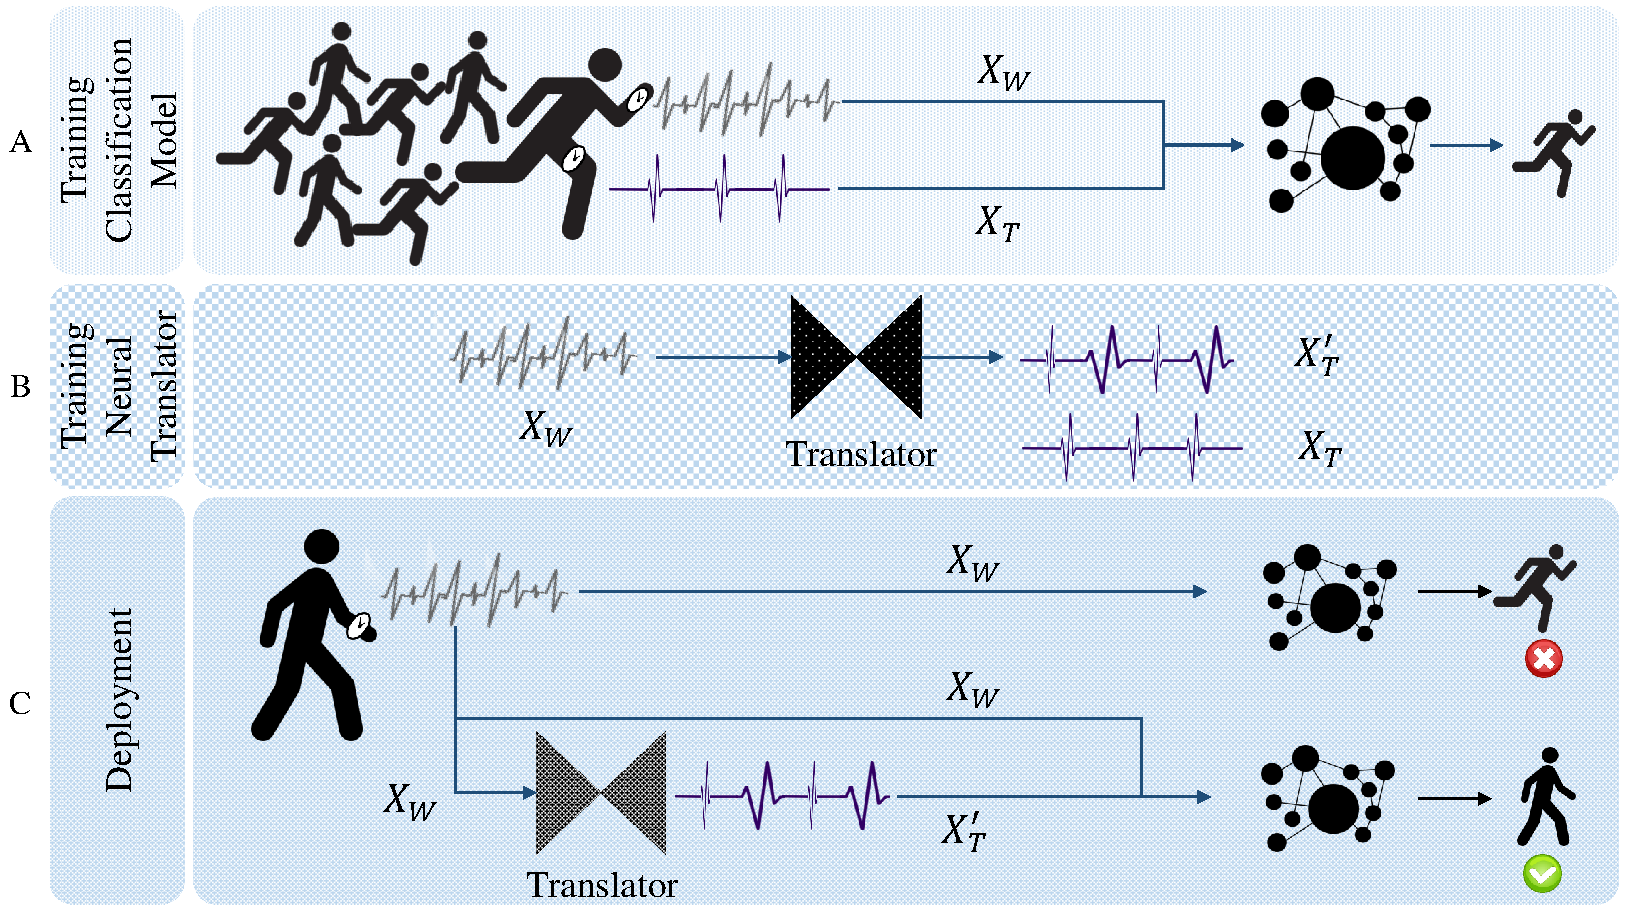
\includegraphics[width=1\textwidth]{e.pdf}
\caption{Improving HAR with Translators}
\label {fig:tran}
\end{figure}
We explored this challenge as a Privileged Learning (PL)~\cite{vapnik2009new} problem where the model is trained with a combination of non-intrusive and intrusive modalities (i. e., ``privileged'' modalities) at training time, but deployed with only non-intrusive modalities. 
Here at deployment, privileged sensor modalities are missing and we look at generative models to replace missing modalities after deployment. 
To this end we introduced two translation approaches that can be used to generate missing or ``privileged" modalities after deployment to augment feature representations and improve HAR.

Figure~\ref{fig:tran} illustrate our approach with two accelerometer sensors on wrist and thigh; where wrist sensor is non-invasive and thigh sensor is invasive in real-time. At training stage we train our classification algorithm with input from both sensors; simultaneously we train a translator to translate between wrist and thigh sensors. After deployment, the user only wears the non-invasive wrist sensor; the classification algorithm is exploiting generated sensor data from our pre-trained translator to emulate the presence of a thigh sensor and performs optimally.
We evaluated the contribution of translators towards the improvement of feature representations with a kNN classifier. We chose kNN as it is a similarity based non-parametric classification algorithm where we can interpret classification results. 
Our results on two HAR datasets, SelfBACK and PAMAP2 showed up-to $5\%$ performance improvement when using representations augmented with translated privileged modalities.
These results suggest that non-intrusive modalities suited for deployment benefit from translation models that generates feature representations that are closer to intrusive modalities.
Full publication for this task including detailed translator methods, evaluation and results can be found on Appendix~\ref{apndx:translators}. 

\subsection{Objective 4 - Zero-Shot Learning with Matching Networks for Open-Ended HAR}
\begin{figure}[ht]
\centering
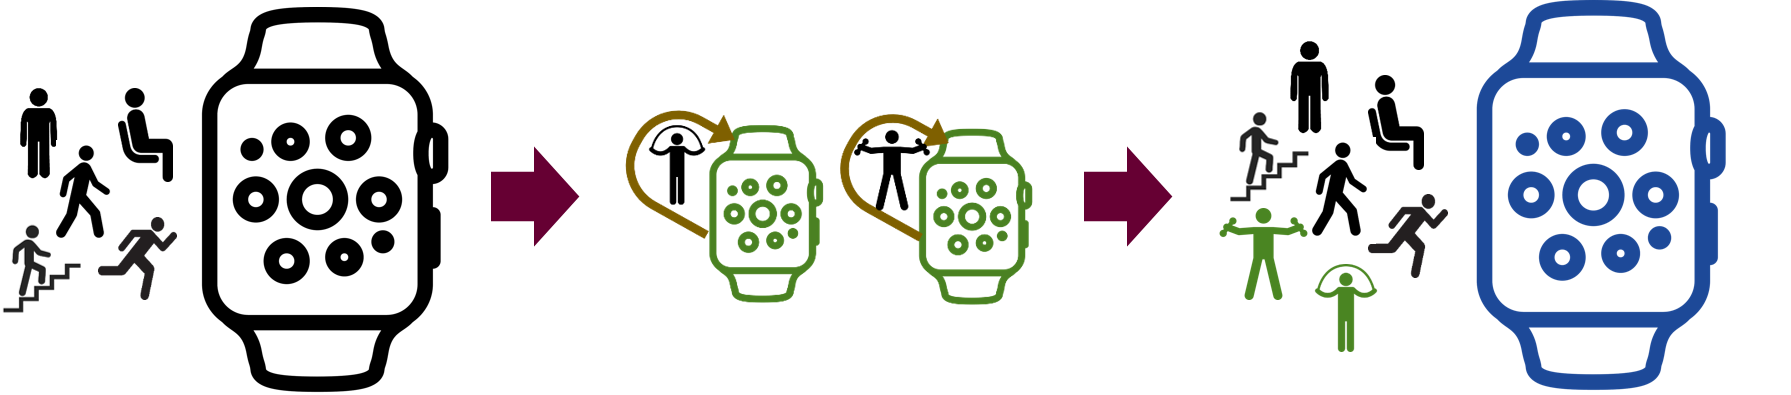
\includegraphics[width=0.9\textwidth]{oehar.png}
\caption{Open-ended HAR with Matching Networks}
\label {fig:oehar}
\end{figure}
Existing Zero-Shot Learning (ZSL) algorithms in the context of open-ended HAR are heavily reliant on expert domain knowledge, which introduces a demanding knowledge acquisition task. 
We proposed to extract a few seconds of raw calibration sensor data, which can be conveniently obtained from micro-interactions with the user, to replace expert domain knowledge.
Figure~\ref{fig:oehar} illustrates our approach to open-ended HAR with ZSL. 
Imagine a fitness application that is only able to recognise a few common activities (e.g. walking, running, sitting) modelled on a general population at design time.
User \textit{A} wants the application to automatically recognise activities they perform regularly but are not packaged in the generic design such as rope jumping and dumbbell exercises. 
They records a few seconds of calibration data for each new activity using sensors available on the wearable device. Subsequently the application extend its functionality into recognising these new activities using calibration data (sensor and activity label) in the future. 

Our approach is based on Matching Networks~\cite{vinyals2016matching} architecture, that exploits similarities between this calibration data to perform open-ended HAR. We improve this architecture to evolve as new activities are introduced after deployment. It is noteworthy that this reasoning model is not re-trained with calibration data obtained for new activities after deployment. 
To evaluate the performance of our algorithm, we conducted a comparative study on three HAR datasets. 
Our results confirmed that, with just 5 seconds of calibration data, our approach performs $14- 18\%$ better when compared to recent ZSL algorithms that utilise domain expert input. 
In addition, our results emphasised the need for strategic selection of multiple sensors for reliable Open-ended HAR.
Full details of method, evaluation and results can be found on Appendix~\ref{apndx:openendedhar}. 
\clearpage

\section{Future work}
\label{sec:fut}

One of the main tasks in the future is to evaluate objectives 3 and 4 with remaining datasets and MEx once objective 1 is complete. Therefore completion of Objective 1 is crucial to the timely progress of this research. 
Next we will look at proposed approaches for objectives 2 and 5.

\subsection{Objective 2 - Multi-modal sensor fusion}
As we try to recognise more complex activities, we require multiple sensors with more sophisticated sensor data to observe different aspects of human movement. Reasoning with multiple sensors is challenging specifically when there are multiple data types. In addition it is advantages if the reasoning model can dynamically select the most informative features from all available sensors at each classification instance.
We plan to explore an attention based fusion mechanisms to address this challenge. 
First we will investigate how each sensor modality contributes towards the classification performance of human activities and then explore how a sensor fusion architecture can contribute toward improving previous results. Next we will explore the informed selection of sensors with an attention mechanism. This is inspired by the fact that some sensors may intercept an activity better than others. Attention can be interpreted in different abstraction levels. For instance, first level is informed selection of subset of sensors for a given activity; second level is informed selection of features from the feature representations. We will explore these techniques by generating feature embeddings at several abstract levels with deep feature extraction techniques for each modality. The goal is to attain the most informative features from different sensors to improve recognition of an activity. The expected solution is expected to work with a range of sensors and it should recognise a range of activities from different domains of human activities. 

\subsection{Objective 5 - Similarity based Qualitative HAR}
Qualitative recognition is imperative for an end-to-end real-world application of HAR. We focus on exercises in this objective where qualitative recognition is most advantages and aligns with our goal.
First task is defining quality metrics of exercise performance. Specifically the deviation between expected and actual performance will form the basis for these metrics.
We will look at how deep models can learn differences from spatio-temporal data that belongs to one classification class and evaluate quality difference. This will call for similarity measures in different abstract levels of feature representations. In order to locate differences in finer detail we will treat exercises as a sequence of primitive actions. Here the idea is to isolate the differences with respect to a primitive action rather than modelling a binary decision making task as we saw with~\cite{chen2013rehabilitation}. We plan to explore deep metric learning~\cite{chopra2005learning,hoffer2015deep} techniques to address this challenge.
\clearpage

\section{Time Management Plan}
\label{sec:time}
\begin{figure}[ht]
\centering
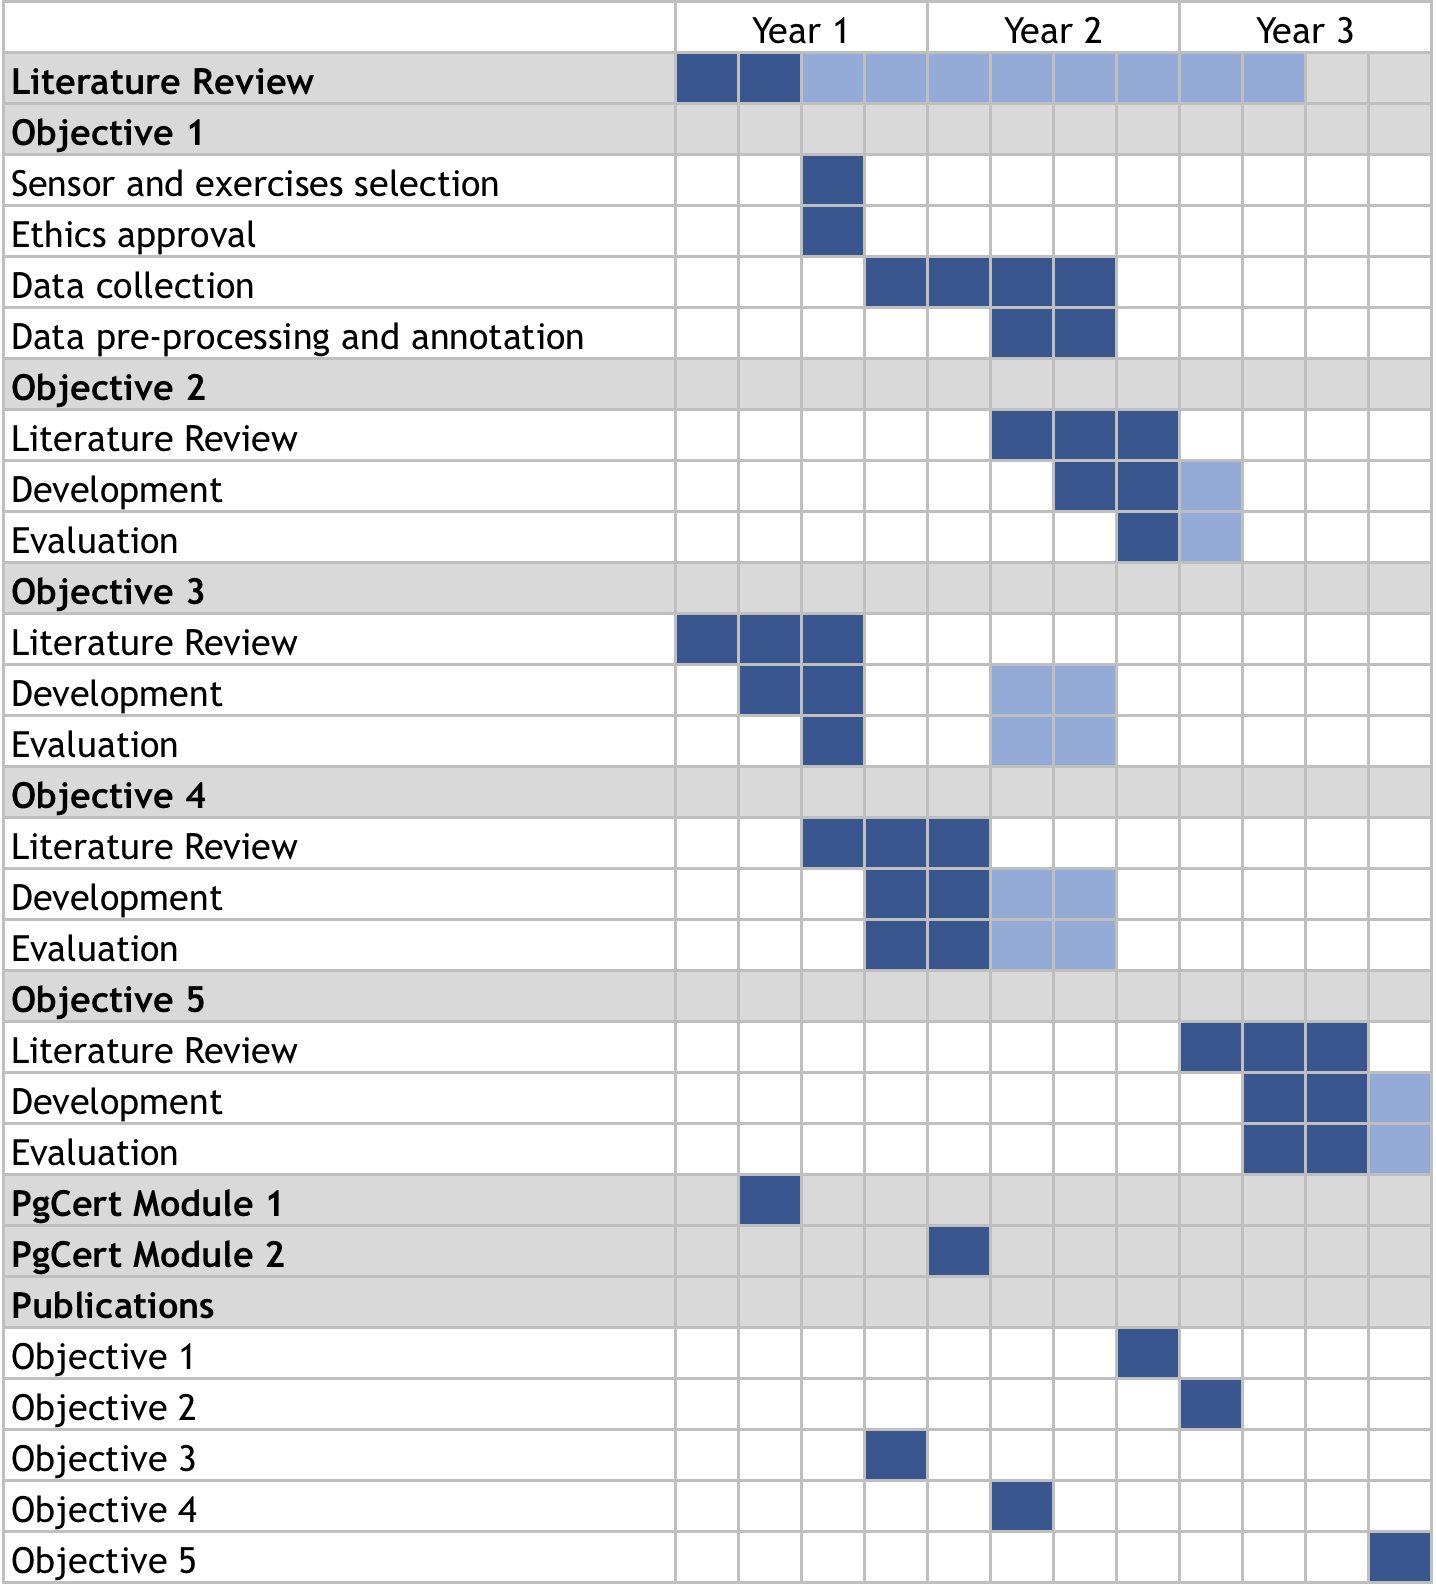
\includegraphics[width=0.8\textwidth]{plan.png}
\caption{Time Management Plan}
\end{figure}

\clearpage

\bibliographystyle{splncs04}
\bibliography{ref}

\begin{appendices}
\section{Improving kNN for Human Activity Recognition with Privileged Learning using Translation Models}
\label{apndx:translators}
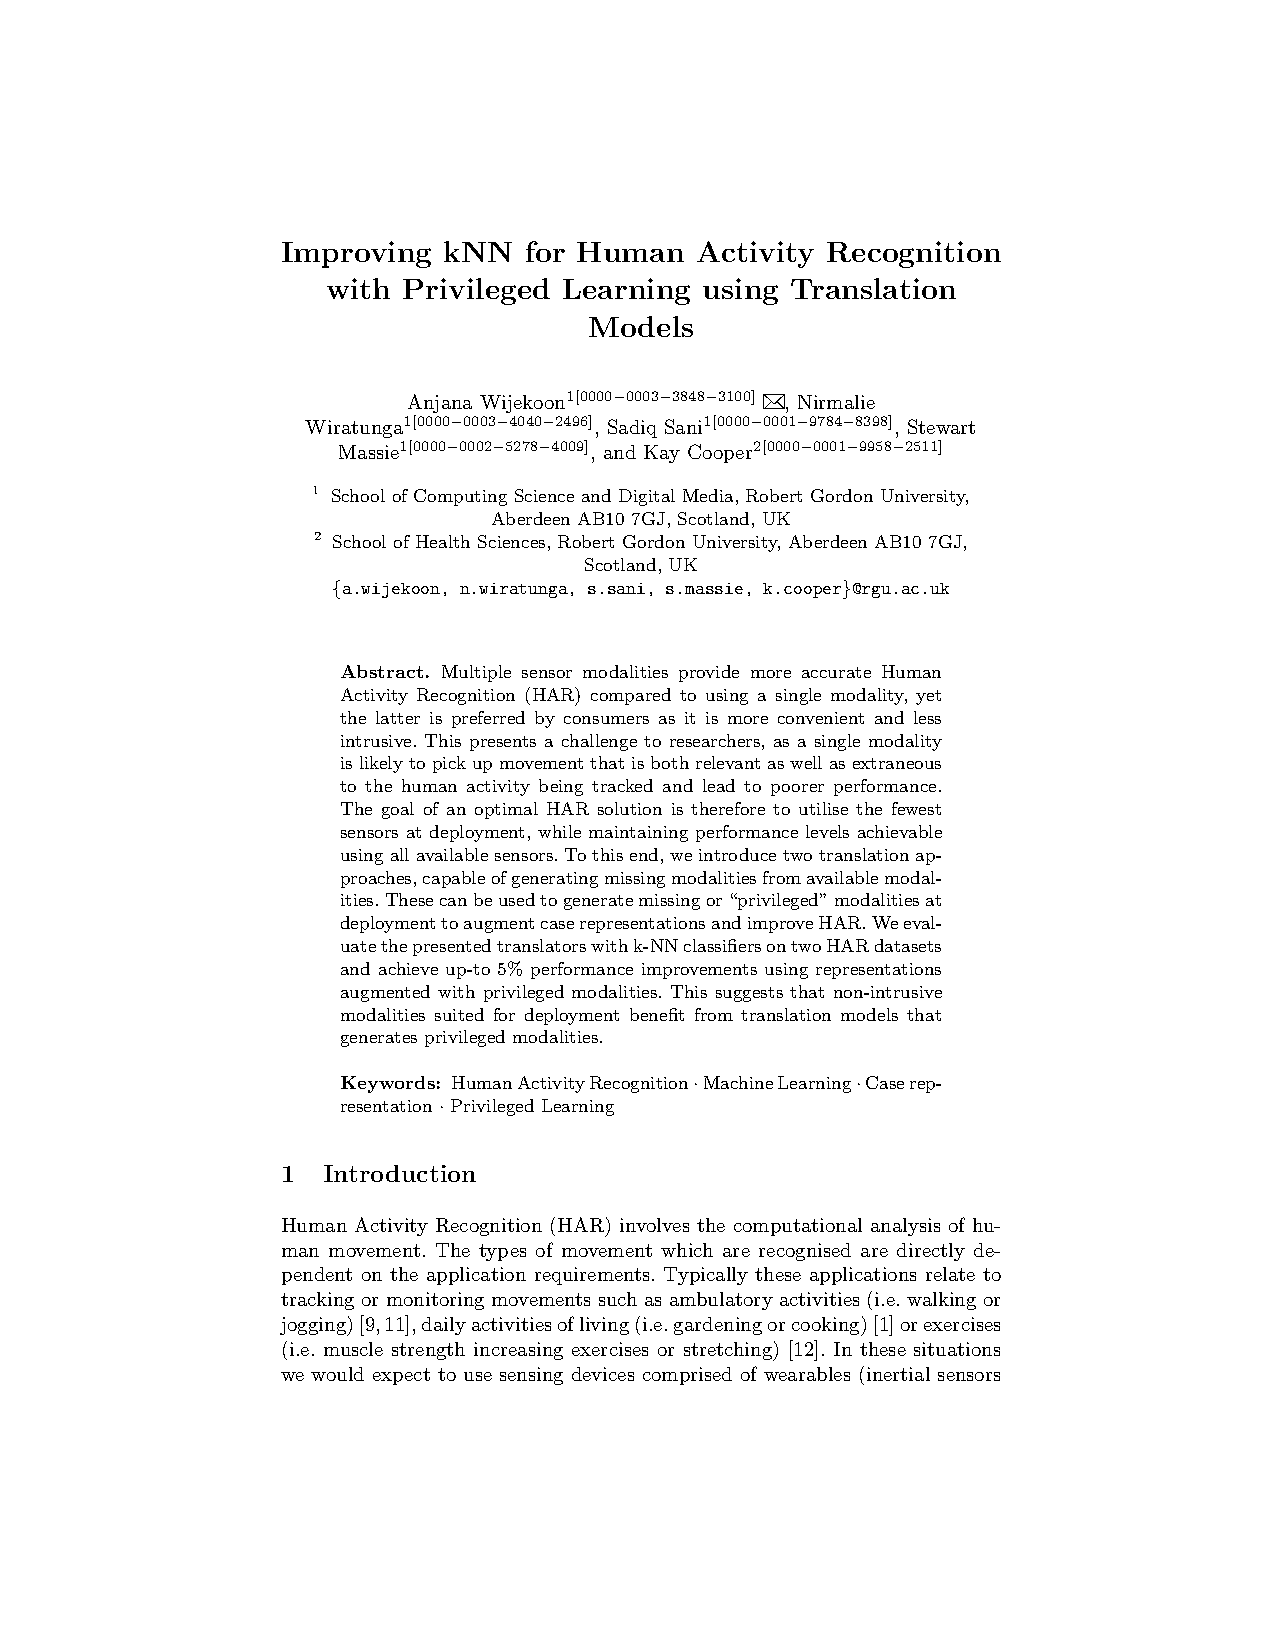
\includepdf[pages=1-]{ICCBR_18.pdf}

\section{Open-Ended Human Activity Recognition using Matching Networks}
\label{apndx:openendedhar}
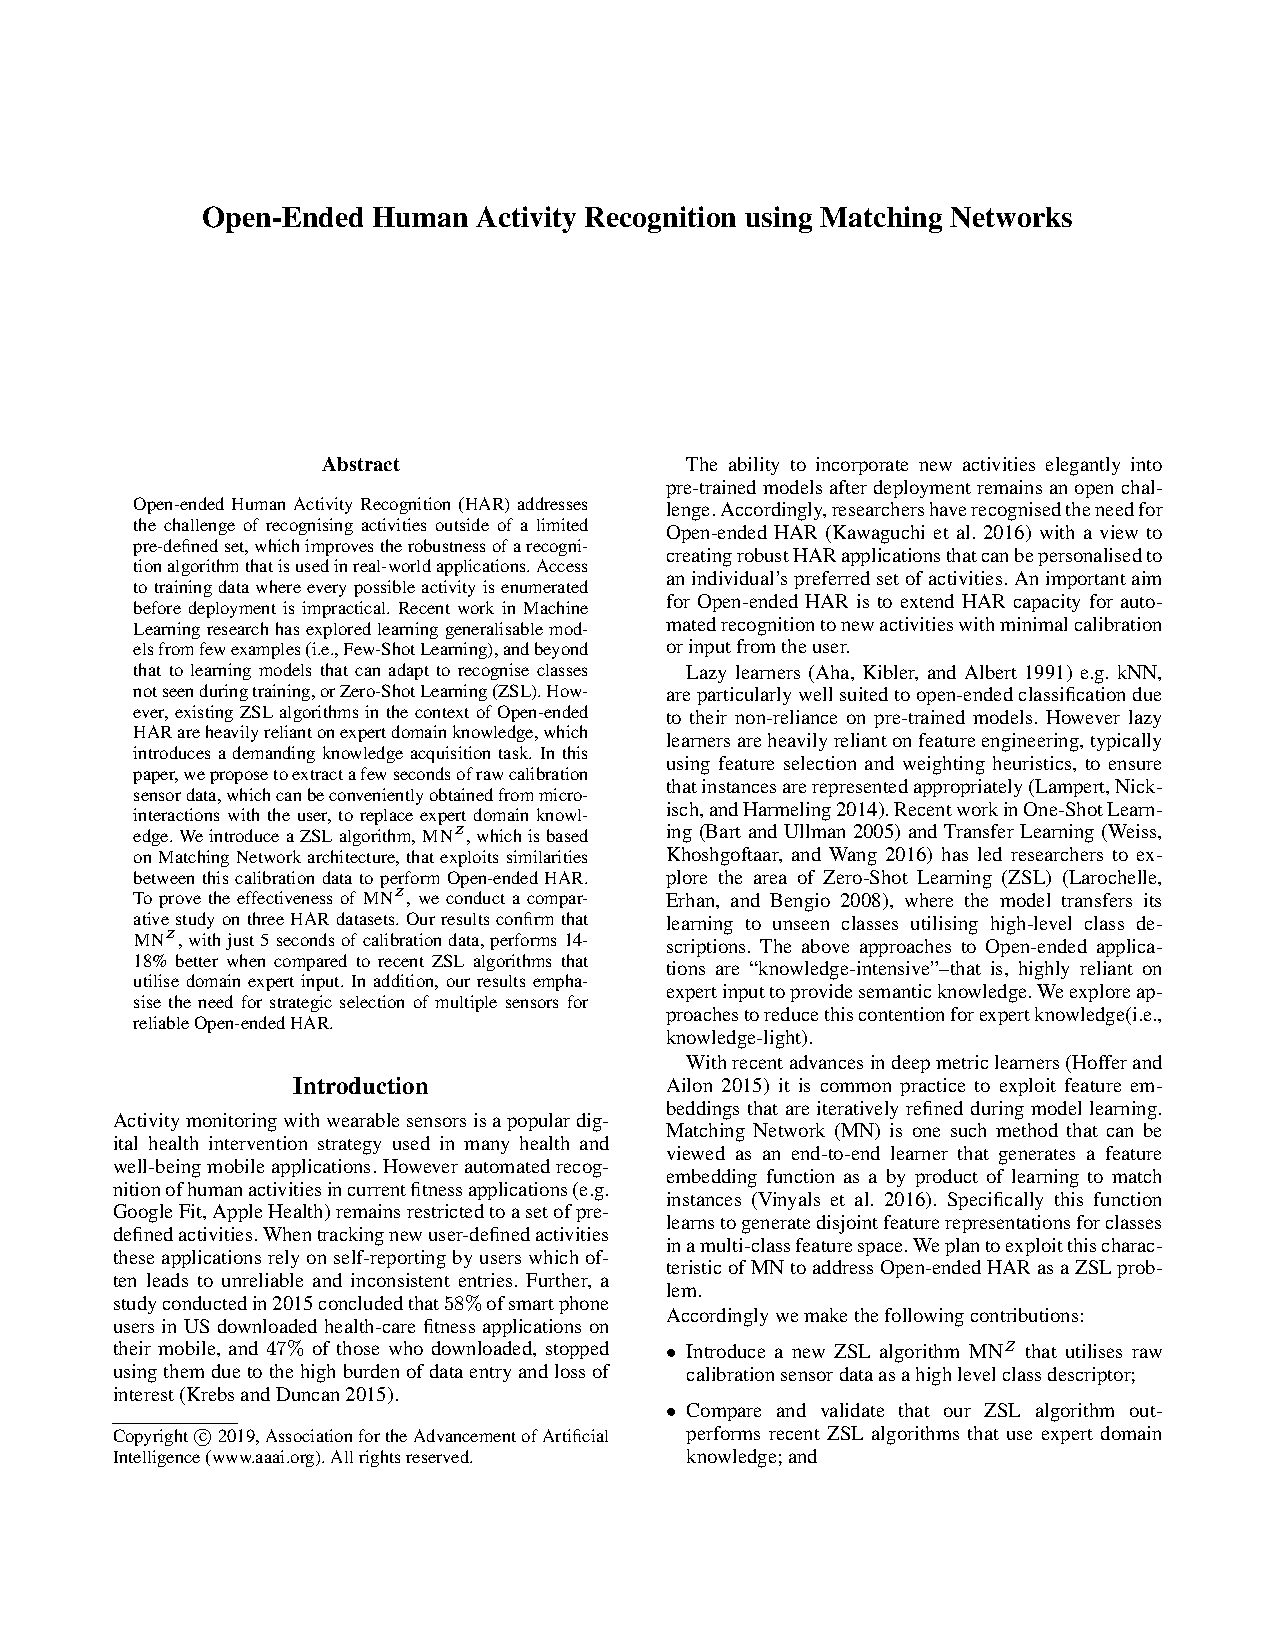
\includepdf[pages=1-]{ZSL_draft.pdf}

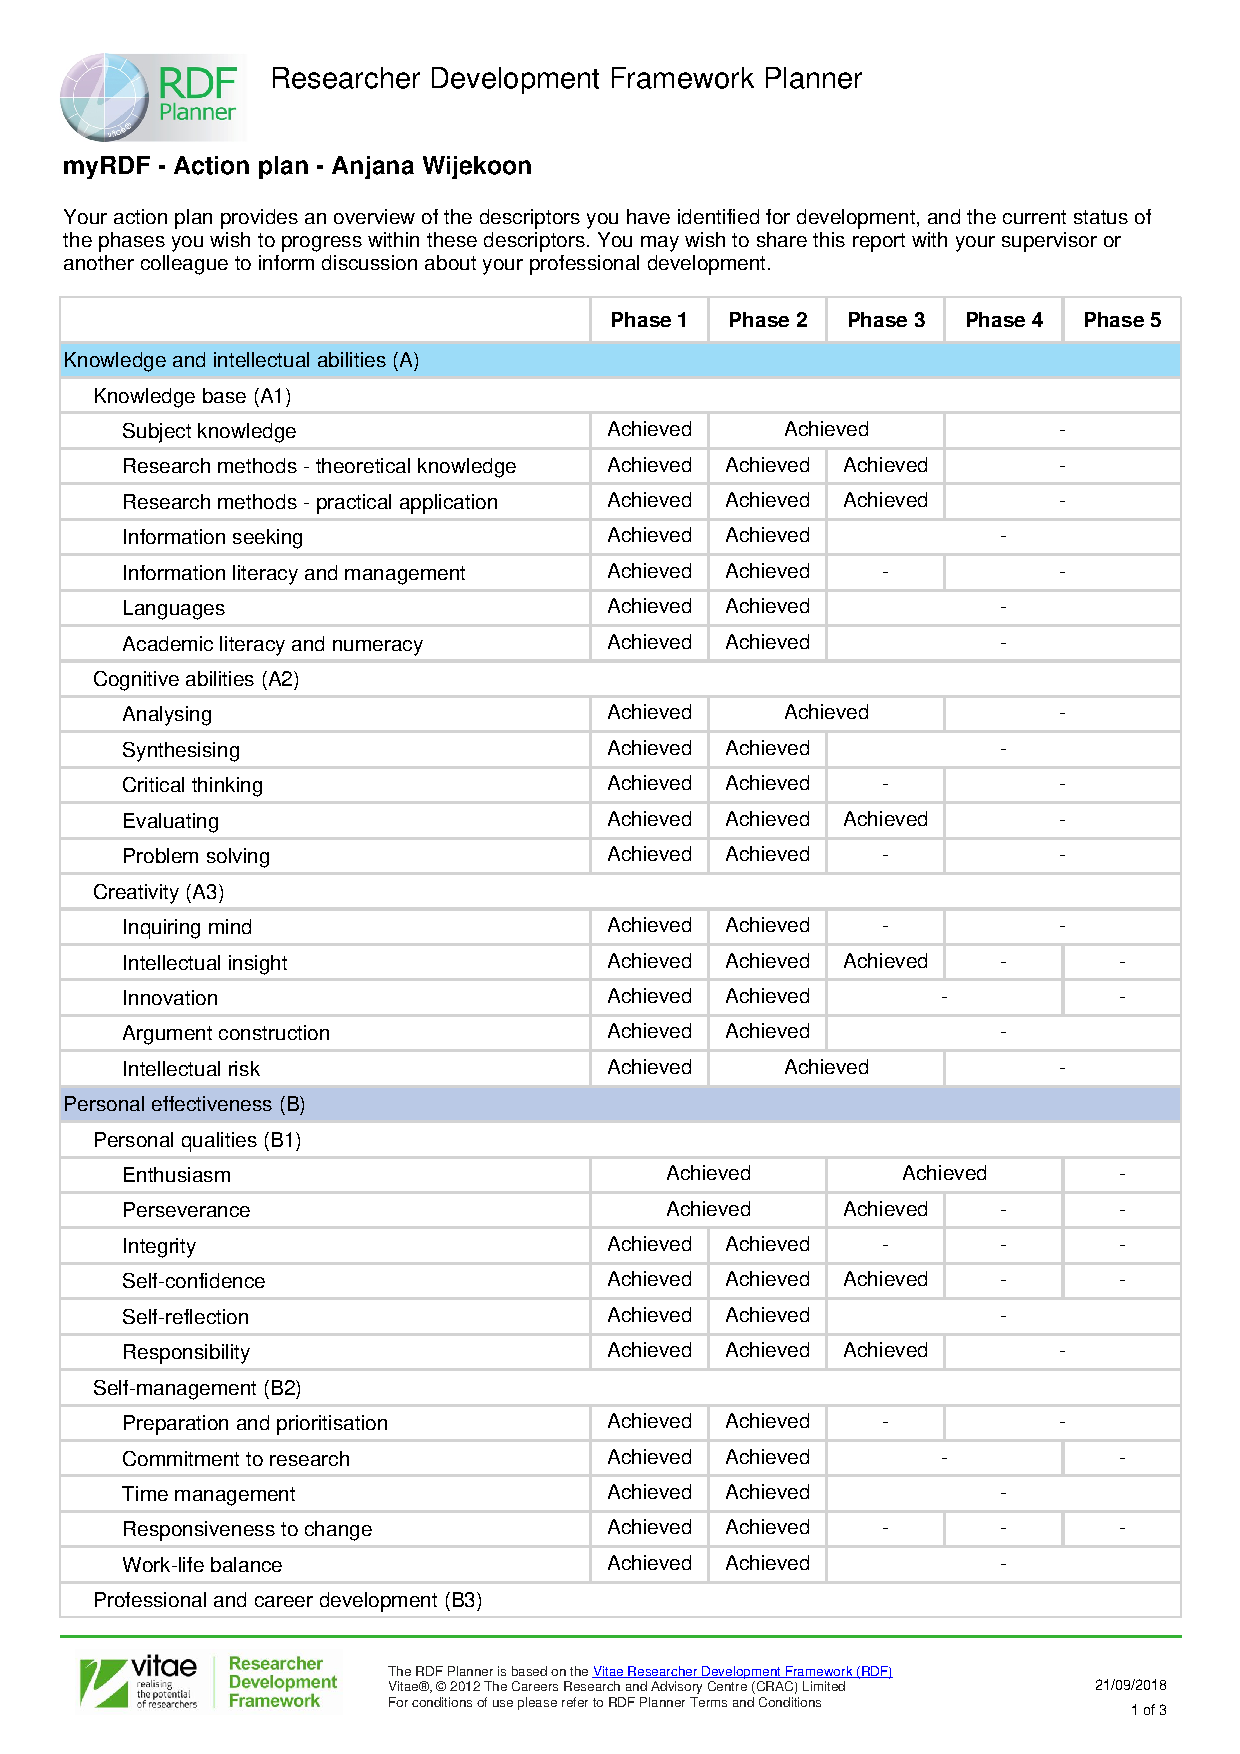
\includepdf[pages=1-]{vitae.pdf}
\end{appendices}

\end{document}

